\documentclass[twoside]{book}

% Packages required by doxygen
\usepackage{fixltx2e}
\usepackage{calc}
\usepackage{doxygen}
\usepackage[export]{adjustbox} % also loads graphicx
\usepackage{graphicx}
\usepackage[utf8]{inputenc}
\usepackage{makeidx}
\usepackage{multicol}
\usepackage{multirow}
\PassOptionsToPackage{warn}{textcomp}
\usepackage{textcomp}
\usepackage[nointegrals]{wasysym}
\usepackage[table]{xcolor}

% Font selection
\usepackage[T1]{fontenc}
\usepackage[scaled=.90]{helvet}
\usepackage{courier}
\usepackage{amssymb}
\usepackage{sectsty}
\renewcommand{\familydefault}{\sfdefault}
\allsectionsfont{%
  \fontseries{bc}\selectfont%
  \color{darkgray}%
}
\renewcommand{\DoxyLabelFont}{%
  \fontseries{bc}\selectfont%
  \color{darkgray}%
}
\newcommand{\+}{\discretionary{\mbox{\scriptsize$\hookleftarrow$}}{}{}}

% Page & text layout
\usepackage{geometry}
\geometry{%
  a4paper,%
  top=2.5cm,%
  bottom=2.5cm,%
  left=2.5cm,%
  right=2.5cm%
}
\tolerance=750
\hfuzz=15pt
\hbadness=750
\setlength{\emergencystretch}{15pt}
\setlength{\parindent}{0cm}
\setlength{\parskip}{0.2cm}
\makeatletter
\renewcommand{\paragraph}{%
  \@startsection{paragraph}{4}{0ex}{-1.0ex}{1.0ex}{%
    \normalfont\normalsize\bfseries\SS@parafont%
  }%
}
\renewcommand{\subparagraph}{%
  \@startsection{subparagraph}{5}{0ex}{-1.0ex}{1.0ex}{%
    \normalfont\normalsize\bfseries\SS@subparafont%
  }%
}
\makeatother

% Headers & footers
\usepackage{fancyhdr}
\pagestyle{fancyplain}
\fancyhead[LE]{\fancyplain{}{\bfseries\thepage}}
\fancyhead[CE]{\fancyplain{}{}}
\fancyhead[RE]{\fancyplain{}{\bfseries\leftmark}}
\fancyhead[LO]{\fancyplain{}{\bfseries\rightmark}}
\fancyhead[CO]{\fancyplain{}{}}
\fancyhead[RO]{\fancyplain{}{\bfseries\thepage}}
\fancyfoot[LE]{\fancyplain{}{}}
\fancyfoot[CE]{\fancyplain{}{}}
\fancyfoot[RE]{\fancyplain{}{\bfseries\scriptsize Generated on Sat Sep 26 2015 14\+:21\+:40 for Windows-\/\+Phone-\/\+Bundle by Doxygen }}
\fancyfoot[LO]{\fancyplain{}{\bfseries\scriptsize Generated on Sat Sep 26 2015 14\+:21\+:40 for Windows-\/\+Phone-\/\+Bundle by Doxygen }}
\fancyfoot[CO]{\fancyplain{}{}}
\fancyfoot[RO]{\fancyplain{}{}}
\renewcommand{\footrulewidth}{0.4pt}
\renewcommand{\chaptermark}[1]{%
  \markboth{#1}{}%
}
\renewcommand{\sectionmark}[1]{%
  \markright{\thesection\ #1}%
}

% Indices & bibliography
\usepackage{natbib}
\usepackage[titles]{tocloft}
\setcounter{tocdepth}{3}
\setcounter{secnumdepth}{5}
\makeindex

% Custom commands
\newcommand{\clearemptydoublepage}{%
  \newpage{\pagestyle{empty}\cleardoublepage}%
}


%===== C O N T E N T S =====

\begin{document}

% Titlepage & ToC
\pagenumbering{roman}
\begin{titlepage}
\vspace*{7cm}
\begin{center}%
{\Large Windows-\/\+Phone-\/\+Bundle }\\
\vspace*{1cm}
{\large Generated by Doxygen 1.8.10}\\
\vspace*{0.5cm}
{\small Sat Sep 26 2015 14:21:40}\\
\end{center}
\end{titlepage}
\clearemptydoublepage
\tableofcontents
\clearemptydoublepage
\pagenumbering{arabic}

%--- Begin generated contents ---
\chapter{Windows-\/\+Phone-\/\+Bundle}
\label{md__r_e_a_d_m_e}
Windows Phone Inplementation of Android.\+os.\+Bundle 
\chapter{Namespace Index}
\section{Packages}
Here are the packages with brief descriptions (if available)\+:\begin{DoxyCompactList}
\item\contentsline{section}{{\bf Bundle\+\_\+\+Library} }{\pageref{namespace_bundle___library}}{}
\item\contentsline{section}{{\bf Bundle\+Test\+App} }{\pageref{namespace_bundle_test_app}}{}
\item\contentsline{section}{{\bf Bundle\+Test\+App.\+Bundle\+Test\+App\+\_\+\+Xaml\+Type\+Info} }{\pageref{namespace_bundle_test_app_1_1_bundle_test_app___xaml_type_info}}{}
\end{DoxyCompactList}

\chapter{Hierarchical Index}
\section{Class Hierarchy}
This inheritance list is sorted roughly, but not completely, alphabetically\+:\begin{DoxyCompactList}
\item Application\begin{DoxyCompactList}
\item \contentsline{section}{Bundle\+Test\+App.\+App}{\pageref{class_bundle_test_app_1_1_app}}{}
\item \contentsline{section}{Bundle\+Test\+App.\+App}{\pageref{class_bundle_test_app_1_1_app}}{}
\item \contentsline{section}{Bundle\+Test\+App.\+App}{\pageref{class_bundle_test_app_1_1_app}}{}
\item \contentsline{section}{Bundle\+Test\+App.\+App}{\pageref{class_bundle_test_app_1_1_app}}{}
\item \contentsline{section}{Bundle\+Test\+App.\+App}{\pageref{class_bundle_test_app_1_1_app}}{}
\end{DoxyCompactList}
\item Exception\begin{DoxyCompactList}
\item \contentsline{section}{Bundle\+\_\+\+Library.\+Invalid\+Bundle\+Exception}{\pageref{class_bundle___library_1_1_invalid_bundle_exception}}{}
\begin{DoxyCompactList}
\item \contentsline{section}{Bundle\+\_\+\+Library.\+Invalid\+Key\+Exception}{\pageref{class_bundle___library_1_1_invalid_key_exception}}{}
\end{DoxyCompactList}
\end{DoxyCompactList}
\item \contentsline{section}{Bundle\+\_\+\+Library.\+I\+Bundleable}{\pageref{interface_bundle___library_1_1_i_bundleable}}{}
\begin{DoxyCompactList}
\item \contentsline{section}{Bundle\+\_\+\+Library.\+Bundle}{\pageref{class_bundle___library_1_1_bundle}}{}
\item \contentsline{section}{Bundle\+\_\+\+Library.\+Test\+Bundleable}{\pageref{class_bundle___library_1_1_test_bundleable}}{}
\end{DoxyCompactList}
\item I\+Component\+Connector\begin{DoxyCompactList}
\item \contentsline{section}{Bundle\+Test\+App.\+App}{\pageref{class_bundle_test_app_1_1_app}}{}
\item \contentsline{section}{Bundle\+Test\+App.\+App}{\pageref{class_bundle_test_app_1_1_app}}{}
\item \contentsline{section}{Bundle\+Test\+App.\+Main\+Page}{\pageref{class_bundle_test_app_1_1_main_page}}{}
\item \contentsline{section}{Bundle\+Test\+App.\+Main\+Page}{\pageref{class_bundle_test_app_1_1_main_page}}{}
\end{DoxyCompactList}
\item I\+Xaml\+Metadata\+Provider\begin{DoxyCompactList}
\item \contentsline{section}{Bundle\+Test\+App.\+App}{\pageref{class_bundle_test_app_1_1_app}}{}
\item \contentsline{section}{Bundle\+Test\+App.\+App}{\pageref{class_bundle_test_app_1_1_app}}{}
\end{DoxyCompactList}
\item Page\begin{DoxyCompactList}
\item \contentsline{section}{Bundle\+Test\+App.\+Main\+Page}{\pageref{class_bundle_test_app_1_1_main_page}}{}
\item \contentsline{section}{Bundle\+Test\+App.\+Main\+Page}{\pageref{class_bundle_test_app_1_1_main_page}}{}
\item \contentsline{section}{Bundle\+Test\+App.\+Main\+Page}{\pageref{class_bundle_test_app_1_1_main_page}}{}
\item \contentsline{section}{Bundle\+Test\+App.\+Main\+Page}{\pageref{class_bundle_test_app_1_1_main_page}}{}
\item \contentsline{section}{Bundle\+Test\+App.\+Main\+Page}{\pageref{class_bundle_test_app_1_1_main_page}}{}
\end{DoxyCompactList}
\end{DoxyCompactList}

\chapter{Class Index}
\section{Class List}
Here are the classes, structs, unions and interfaces with brief descriptions\+:\begin{DoxyCompactList}
\item\contentsline{section}{{\bf Bundle\+Test\+App.\+App} \\*Provides application-\/specific behavior to supplement the default Application class. }{\pageref{class_bundle_test_app_1_1_app}}{}
\item\contentsline{section}{{\bf Bundle\+\_\+\+Library.\+Bundle} \\*This class represents a bundle. A bundle is a collection of other objects all stored together. objects within a bundle can be accessed using the key they were stored under. }{\pageref{class_bundle___library_1_1_bundle}}{}
\item\contentsline{section}{{\bf Bundle\+\_\+\+Library.\+I\+Bundleable} \\*This interface allows objects to be packed in bundles. Any object you want to pack in a bundle must implement this interface }{\pageref{interface_bundle___library_1_1_i_bundleable}}{}
\item\contentsline{section}{{\bf Bundle\+\_\+\+Library.\+Invalid\+Bundle\+Exception} \\*This class represents an exception which is thrown when an invalid bundle has been used for a pack unpack operation }{\pageref{class_bundle___library_1_1_invalid_bundle_exception}}{}
\item\contentsline{section}{{\bf Bundle\+\_\+\+Library.\+Invalid\+Key\+Exception} \\*This class represents an exception which is thrown when the key was not found within the bundle }{\pageref{class_bundle___library_1_1_invalid_key_exception}}{}
\item\contentsline{section}{{\bf Bundle\+Test\+App.\+Main\+Page} \\*An empty page that can be used on its own or navigated to within a Frame. }{\pageref{class_bundle_test_app_1_1_main_page}}{}
\item\contentsline{section}{{\bf Bundle\+\_\+\+Library.\+Test\+Bundleable} \\*This class represents a simple object that can be packed and unpacked from a bundle. }{\pageref{class_bundle___library_1_1_test_bundleable}}{}
\end{DoxyCompactList}

\chapter{Namespace Documentation}
\section{Bundle\+\_\+\+Library Namespace Reference}
\label{namespace_bundle___library}\index{Bundle\+\_\+\+Library@{Bundle\+\_\+\+Library}}
\subsection*{Classes}
\begin{DoxyCompactItemize}
\item 
class {\bf Bundle}
\begin{DoxyCompactList}\small\item\em This class represents a bundle. A bundle is a collection of other objects all stored together. objects within a bundle can be accessed using the key they were stored under. \end{DoxyCompactList}\item 
interface {\bf I\+Bundleable}
\begin{DoxyCompactList}\small\item\em This interface allows objects to be packed in bundles. Any object you want to pack in a bundle must implement this interface \end{DoxyCompactList}\item 
class {\bf Invalid\+Bundle\+Exception}
\begin{DoxyCompactList}\small\item\em This class represents an exception which is thrown when an invalid bundle has been used for a pack unpack operation \end{DoxyCompactList}\item 
class {\bf Invalid\+Key\+Exception}
\begin{DoxyCompactList}\small\item\em This class represents an exception which is thrown when the key was not found within the bundle \end{DoxyCompactList}\end{DoxyCompactItemize}

\section{Bundle\+Test\+App Namespace Reference}
\label{namespace_bundle_test_app}\index{Bundle\+Test\+App@{Bundle\+Test\+App}}
\subsection*{Namespaces}
\begin{DoxyCompactItemize}
\item 
namespace {\bf Bundle\+Test\+App\+\_\+\+Xaml\+Type\+Info}
\end{DoxyCompactItemize}
\subsection*{Classes}
\begin{DoxyCompactItemize}
\item 
class {\bf App}
\begin{DoxyCompactList}\small\item\em Provides application-\/specific behavior to supplement the default Application class. \end{DoxyCompactList}\item 
class {\bf Main\+Page}
\begin{DoxyCompactList}\small\item\em An empty page that can be used on its own or navigated to within a Frame. \end{DoxyCompactList}\item 
class {\bfseries Program}
\end{DoxyCompactItemize}

\section{Bundle\+Test\+App.\+Bundle\+Test\+App\+\_\+\+Xaml\+Type\+Info Namespace Reference}
\label{namespace_bundle_test_app_1_1_bundle_test_app___xaml_type_info}\index{Bundle\+Test\+App.\+Bundle\+Test\+App\+\_\+\+Xaml\+Type\+Info@{Bundle\+Test\+App.\+Bundle\+Test\+App\+\_\+\+Xaml\+Type\+Info}}
\subsection*{Classes}
\begin{DoxyCompactItemize}
\item 
class {\bfseries Xaml\+Member}
\item 
class {\bfseries Xaml\+System\+Base\+Type}
\item 
class {\bfseries Xaml\+Type\+Info\+Provider}
\item 
class {\bfseries Xaml\+User\+Type}
\end{DoxyCompactItemize}

\chapter{Class Documentation}
\section{Bundle\+Test\+App.\+App Class Reference}
\label{class_bundle_test_app_1_1_app}\index{Bundle\+Test\+App.\+App@{Bundle\+Test\+App.\+App}}


Provides application-\/specific behavior to supplement the default Application class.  


Inheritance diagram for Bundle\+Test\+App.\+App\+:\begin{figure}[H]
\begin{center}
\leavevmode
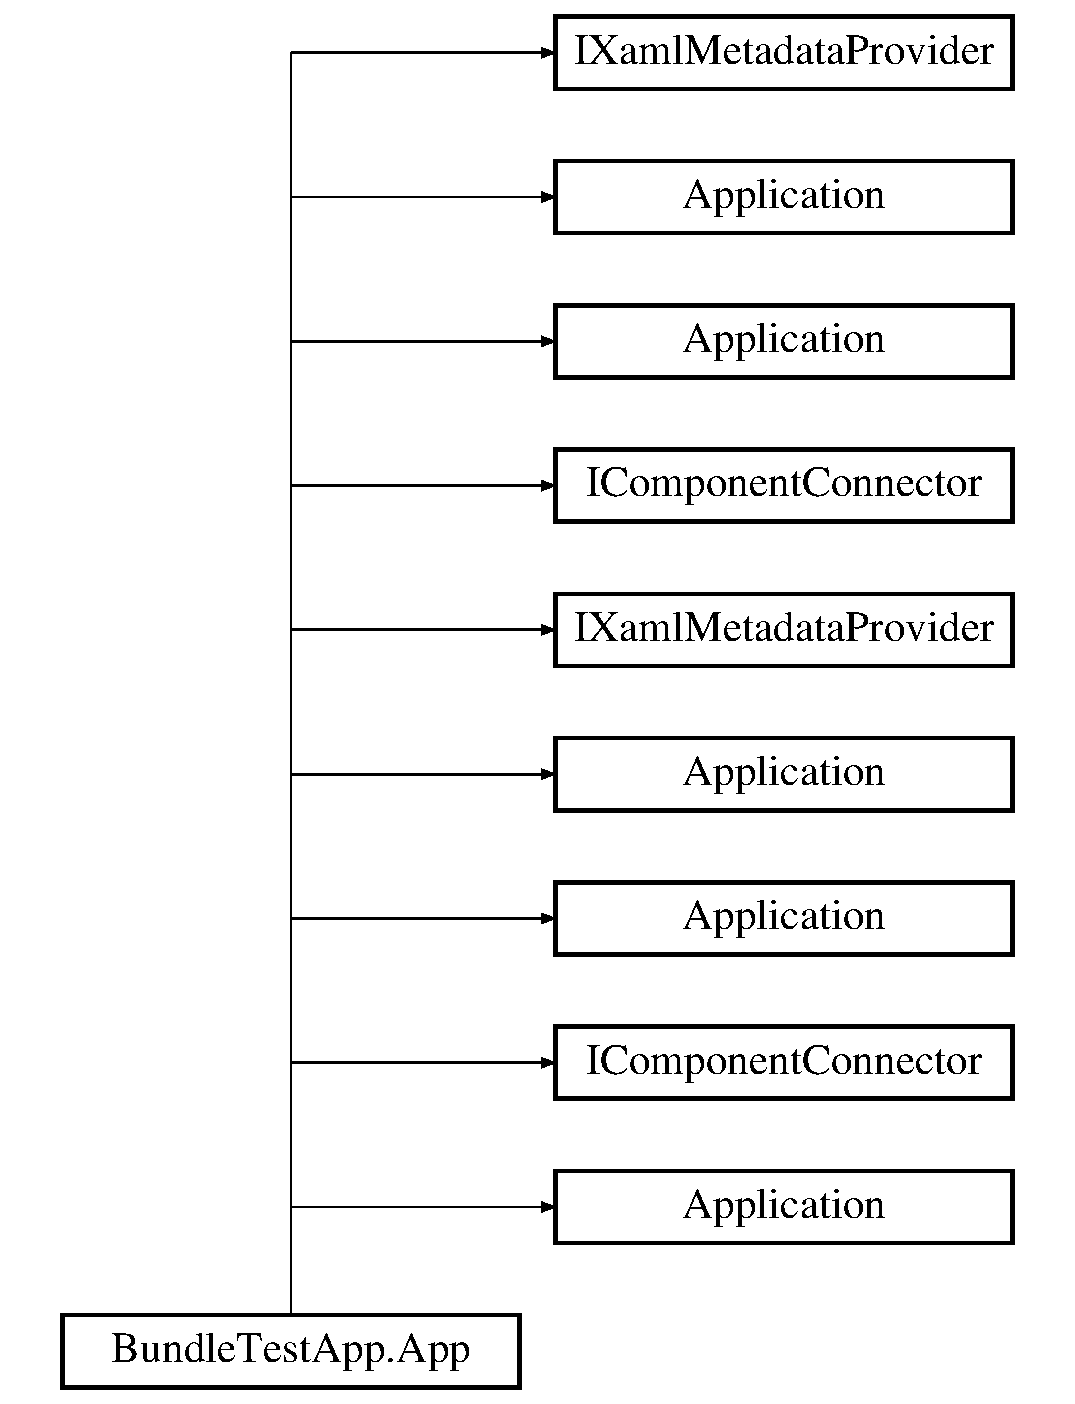
\includegraphics[height=10.000000cm]{class_bundle_test_app_1_1_app}
\end{center}
\end{figure}
\subsection*{Public Member Functions}
\begin{DoxyCompactItemize}
\item 
{\bf App} ()
\begin{DoxyCompactList}\small\item\em Initializes the singleton application object. This is the first line of authored code executed, and as such is the logical equivalent of main() or Win\+Main(). \end{DoxyCompactList}\item 
void {\bfseries Connect} (int connection\+Id, object target)\label{class_bundle_test_app_1_1_app_a0a5635d86e70a262031ceba6403a0f09}

\item 
void {\bfseries Initialize\+Component} ()\label{class_bundle_test_app_1_1_app_aa68b4e421fa0219b98819c91082d7885}

\item 
global\+::\+Windows.\+U\+I.\+Xaml.\+Markup.\+I\+Xaml\+Type {\bfseries Get\+Xaml\+Type} (global\+::\+System.\+Type type)\label{class_bundle_test_app_1_1_app_a2ce321b9da23883ba14f16b34da5169f}

\item 
global\+::\+Windows.\+U\+I.\+Xaml.\+Markup.\+I\+Xaml\+Type {\bfseries Get\+Xaml\+Type} (string full\+Name)\label{class_bundle_test_app_1_1_app_aa412ded48806f9e13662001548cd7c3d}

\item 
global\+::\+Windows.\+U\+I.\+Xaml.\+Markup.\+Xmlns\+Definition[$\,$] {\bfseries Get\+Xmlns\+Definitions} ()\label{class_bundle_test_app_1_1_app_a510e2dd8e2de1264eed6f3f35fcbd3be}

\item 
void {\bfseries Connect} (int connection\+Id, object target)\label{class_bundle_test_app_1_1_app_a0a5635d86e70a262031ceba6403a0f09}

\item 
void {\bfseries Initialize\+Component} ()\label{class_bundle_test_app_1_1_app_aa68b4e421fa0219b98819c91082d7885}

\item 
global\+::\+Windows.\+U\+I.\+Xaml.\+Markup.\+I\+Xaml\+Type {\bfseries Get\+Xaml\+Type} (global\+::\+System.\+Type type)\label{class_bundle_test_app_1_1_app_a2ce321b9da23883ba14f16b34da5169f}

\item 
global\+::\+Windows.\+U\+I.\+Xaml.\+Markup.\+I\+Xaml\+Type {\bfseries Get\+Xaml\+Type} (string full\+Name)\label{class_bundle_test_app_1_1_app_aa412ded48806f9e13662001548cd7c3d}

\item 
global\+::\+Windows.\+U\+I.\+Xaml.\+Markup.\+Xmlns\+Definition[$\,$] {\bfseries Get\+Xmlns\+Definitions} ()\label{class_bundle_test_app_1_1_app_a510e2dd8e2de1264eed6f3f35fcbd3be}

\end{DoxyCompactItemize}
\subsection*{Protected Member Functions}
\begin{DoxyCompactItemize}
\item 
override void {\bf On\+Launched} (Launch\+Activated\+Event\+Args e)
\begin{DoxyCompactList}\small\item\em Invoked when the application is launched normally by the end user. Other entry points will be used when the application is launched to open a specific file, to display search results, and so forth. \end{DoxyCompactList}\end{DoxyCompactItemize}


\subsection{Detailed Description}
Provides application-\/specific behavior to supplement the default Application class. 



\subsection{Constructor \& Destructor Documentation}
\index{Bundle\+Test\+App\+::\+App@{Bundle\+Test\+App\+::\+App}!App@{App}}
\index{App@{App}!Bundle\+Test\+App\+::\+App@{Bundle\+Test\+App\+::\+App}}
\subsubsection[{App()}]{\setlength{\rightskip}{0pt plus 5cm}Bundle\+Test\+App.\+App.\+App (
\begin{DoxyParamCaption}
{}
\end{DoxyParamCaption}
)}\label{class_bundle_test_app_1_1_app_a4b1213d9a13b6c3da01c462007db7e15}


Initializes the singleton application object. This is the first line of authored code executed, and as such is the logical equivalent of main() or Win\+Main(). 



\subsection{Member Function Documentation}
\index{Bundle\+Test\+App\+::\+App@{Bundle\+Test\+App\+::\+App}!On\+Launched@{On\+Launched}}
\index{On\+Launched@{On\+Launched}!Bundle\+Test\+App\+::\+App@{Bundle\+Test\+App\+::\+App}}
\subsubsection[{On\+Launched(\+Launch\+Activated\+Event\+Args e)}]{\setlength{\rightskip}{0pt plus 5cm}override void Bundle\+Test\+App.\+App.\+On\+Launched (
\begin{DoxyParamCaption}
\item[{Launch\+Activated\+Event\+Args}]{e}
\end{DoxyParamCaption}
)\hspace{0.3cm}{\ttfamily [protected]}}\label{class_bundle_test_app_1_1_app_a787a50886c11e0a1ecc0a185f2dc3a7e}


Invoked when the application is launched normally by the end user. Other entry points will be used when the application is launched to open a specific file, to display search results, and so forth. 


\begin{DoxyParams}{Parameters}
{\em e} & Details about the launch request and process.\\
\hline
\end{DoxyParams}


The documentation for this class was generated from the following files\+:\begin{DoxyCompactItemize}
\item 
D\+:/\+Git\+Hub/\+Windows-\/\+Phone-\/\+Bundle/\+Bundle\+Test\+App/App.\+xaml.\+cs\item 
D\+:/\+Git\+Hub/\+Windows-\/\+Phone-\/\+Bundle/\+Bundle\+Test\+App/obj/\+Debug/App.\+g.\+i.\+cs\item 
D\+:/\+Git\+Hub/\+Windows-\/\+Phone-\/\+Bundle/\+Bundle\+Test\+App/obj/\+Debug/Xaml\+Type\+Info.\+g.\+cs\item 
D\+:/\+Git\+Hub/\+Windows-\/\+Phone-\/\+Bundle/\+Bundle\+Test\+App/obj/\+Debug/App.\+g.\+cs\end{DoxyCompactItemize}

\section{Bundle\+\_\+\+Library.\+Bundle Class Reference}
\label{class_bundle___library_1_1_bundle}\index{Bundle\+\_\+\+Library.\+Bundle@{Bundle\+\_\+\+Library.\+Bundle}}


This class represents a bundle. A bundle is a collection of other objects all stored together. objects within a bundle can be accessed using the key they were stored under.  


Inheritance diagram for Bundle\+\_\+\+Library.\+Bundle\+:\begin{figure}[H]
\begin{center}
\leavevmode
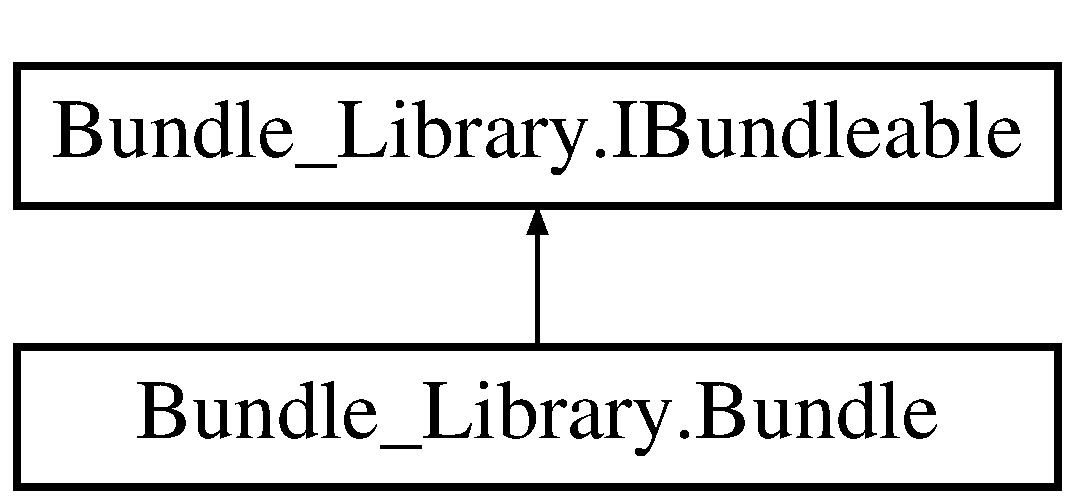
\includegraphics[height=2.000000cm]{class_bundle___library_1_1_bundle}
\end{center}
\end{figure}
\subsection*{Public Member Functions}
\begin{DoxyCompactItemize}
\item 
{\bf Bundle} (string from)
\begin{DoxyCompactList}\small\item\em Default contructor for this bundle \end{DoxyCompactList}\item 
void {\bf pack\+Object} (string key, {\bf Bundle} B)
\begin{DoxyCompactList}\small\item\em Pack this object into a bundle \end{DoxyCompactList}\item 
{\bf I\+Bundleable} {\bf unpack\+Ooject} (string key, {\bf Bundle} B)
\begin{DoxyCompactList}\small\item\em Unpack this object from the bundle \end{DoxyCompactList}\item 
void {\bf store\+Packed\+Object} (string key, {\bf I\+Bundleable} obj)
\begin{DoxyCompactList}\small\item\em Private internal method call used by the \doxyref{I\+Bundleable}{p.}{interface_bundle___library_1_1_i_bundleable} interfaces pack\+Object(key,obj) method \end{DoxyCompactList}\item 
{\bf I\+Bundleable} {\bf get\+Packed\+Object} (string key)
\begin{DoxyCompactList}\small\item\em Private internal method call used by the \doxyref{I\+Bundleable}{p.}{interface_bundle___library_1_1_i_bundleable} interfaces unpack\+Object(key) method \end{DoxyCompactList}\item 
String {\bf get\+String} (string key)
\begin{DoxyCompactList}\small\item\em gets a string from this bundle \end{DoxyCompactList}\item 
int {\bf get\+Int} (string key)
\begin{DoxyCompactList}\small\item\em gets a integer from this bundle \end{DoxyCompactList}\item 
long {\bf get\+Long} (string key)
\begin{DoxyCompactList}\small\item\em gets a long from this bundle \end{DoxyCompactList}\item 
float {\bf get\+Float} (string key)
\begin{DoxyCompactList}\small\item\em gets a float from this bundle \end{DoxyCompactList}\item 
double {\bf get\+Double} (string key)
\begin{DoxyCompactList}\small\item\em gets a double from this bundle \end{DoxyCompactList}\item 
bool {\bf get\+Bool} (string key)
\begin{DoxyCompactList}\small\item\em gets a boolean from this bundle \end{DoxyCompactList}\item 
char {\bf get\+Char} (string key)
\begin{DoxyCompactList}\small\item\em gets a character from this bundle \end{DoxyCompactList}\item 
String[$\,$] {\bf get\+String\+Array} (string key)
\begin{DoxyCompactList}\small\item\em gets a string array from this bundle \end{DoxyCompactList}\item 
int[$\,$] {\bf get\+Int\+Array} (string key)
\begin{DoxyCompactList}\small\item\em gets a integer array from this bundle \end{DoxyCompactList}\item 
long[$\,$] {\bf get\+Long\+Array} (string key)
\begin{DoxyCompactList}\small\item\em gets a long array from this bundle \end{DoxyCompactList}\item 
float[$\,$] {\bf get\+Float\+Array} (string key)
\begin{DoxyCompactList}\small\item\em gets a float array from this bundle \end{DoxyCompactList}\item 
double[$\,$] {\bf get\+Double\+Array} (string key)
\begin{DoxyCompactList}\small\item\em gets a double array from this bundle \end{DoxyCompactList}\item 
bool[$\,$] {\bf get\+Bool\+Arrays} (string key)
\begin{DoxyCompactList}\small\item\em gets a boolean array from this bundle \end{DoxyCompactList}\item 
char[$\,$] {\bf get\+Char\+Arrays} (string key)
\begin{DoxyCompactList}\small\item\em gets a character array from this bundle \end{DoxyCompactList}\item 
void {\bf put\+String} (string key, string value)
\begin{DoxyCompactList}\small\item\em Puts a string into this bundle \end{DoxyCompactList}\item 
void {\bf put\+Int} (string key, int value)
\begin{DoxyCompactList}\small\item\em Puts a integer into this bundle \end{DoxyCompactList}\item 
void {\bf put\+Long} (string key, long value)
\begin{DoxyCompactList}\small\item\em Puts a long into this bundle \end{DoxyCompactList}\item 
void {\bf put\+Float} (string key, float value)
\begin{DoxyCompactList}\small\item\em Puts a float into this bundle \end{DoxyCompactList}\item 
void {\bf put\+Double} (string key, double value)
\begin{DoxyCompactList}\small\item\em Puts a double into this bundle \end{DoxyCompactList}\item 
void {\bf put\+Bool} (string key, bool value)
\begin{DoxyCompactList}\small\item\em Puts a boolean into this bundle \end{DoxyCompactList}\item 
void {\bf put\+Char} (string key, char value)
\begin{DoxyCompactList}\small\item\em Puts a character into this bundle \end{DoxyCompactList}\item 
void {\bf put\+String\+Array} (string key, string[$\,$] value)
\begin{DoxyCompactList}\small\item\em Puts a string array into this bundle \end{DoxyCompactList}\item 
void {\bf put\+Int\+Array} (string key, int[$\,$] value)
\begin{DoxyCompactList}\small\item\em Puts a integer array into this bundle \end{DoxyCompactList}\item 
void {\bf put\+Long\+Array} (string key, long[$\,$] value)
\begin{DoxyCompactList}\small\item\em Puts a long array into this bundle \end{DoxyCompactList}\item 
void {\bf put\+Float\+Array} (string key, float[$\,$] value)
\begin{DoxyCompactList}\small\item\em Puts a float array into this bundle \end{DoxyCompactList}\item 
void {\bf put\+Double\+Array} (string key, double[$\,$] value)
\begin{DoxyCompactList}\small\item\em Puts a double array into this bundle \end{DoxyCompactList}\item 
void {\bf put\+Bool\+Array} (string key, bool[$\,$] value)
\begin{DoxyCompactList}\small\item\em Puts a boolean array into this bundle \end{DoxyCompactList}\item 
void {\bf put\+Char\+Array} (string key, char[$\,$] value)
\begin{DoxyCompactList}\small\item\em Puts a character array into this bundle \end{DoxyCompactList}\end{DoxyCompactItemize}
\subsection*{Static Public Member Functions}
\begin{DoxyCompactItemize}
\item 
static {\bf Bundle} {\bf operator+} ({\bf Bundle} lhs, {\bf Bundle} rhs)
\begin{DoxyCompactList}\small\item\em Custom overload of the binary plus operator which allows two bundle structures to be merged \end{DoxyCompactList}\end{DoxyCompactItemize}
\subsection*{Static Public Attributes}
\begin{DoxyCompactItemize}
\item 
static readonly {\bf Bundle} {\bf E\+M\+P\+T\+Y} = new {\bf Bundle}(\char`\"{}\char`\"{})
\begin{DoxyCompactList}\small\item\em An empty bundle used to check if a bundle is empty \end{DoxyCompactList}\end{DoxyCompactItemize}
\subsection*{Properties}
\begin{DoxyCompactItemize}
\item 
string {\bfseries Identifier}\hspace{0.3cm}{\ttfamily  [get]}\label{class_bundle___library_1_1_bundle_a2bdc262090f95f28789569c5c49241e3}

\end{DoxyCompactItemize}


\subsection{Detailed Description}
This class represents a bundle. A bundle is a collection of other objects all stored together. objects within a bundle can be accessed using the key they were stored under. 



\subsection{Constructor \& Destructor Documentation}
\index{Bundle\+\_\+\+Library\+::\+Bundle@{Bundle\+\_\+\+Library\+::\+Bundle}!Bundle@{Bundle}}
\index{Bundle@{Bundle}!Bundle\+\_\+\+Library\+::\+Bundle@{Bundle\+\_\+\+Library\+::\+Bundle}}
\subsubsection[{Bundle(string from)}]{\setlength{\rightskip}{0pt plus 5cm}Bundle\+\_\+\+Library.\+Bundle.\+Bundle (
\begin{DoxyParamCaption}
\item[{string}]{from}
\end{DoxyParamCaption}
)}\label{class_bundle___library_1_1_bundle_a6f40b35cab88241f77f2df60b4544e91}


Default contructor for this bundle 


\begin{DoxyParams}{Parameters}
{\em from} & string identifier to specify where this bundle came from \\
\hline
\end{DoxyParams}


\subsection{Member Function Documentation}
\index{Bundle\+\_\+\+Library\+::\+Bundle@{Bundle\+\_\+\+Library\+::\+Bundle}!get\+Bool@{get\+Bool}}
\index{get\+Bool@{get\+Bool}!Bundle\+\_\+\+Library\+::\+Bundle@{Bundle\+\_\+\+Library\+::\+Bundle}}
\subsubsection[{get\+Bool(string key)}]{\setlength{\rightskip}{0pt plus 5cm}bool Bundle\+\_\+\+Library.\+Bundle.\+get\+Bool (
\begin{DoxyParamCaption}
\item[{string}]{key}
\end{DoxyParamCaption}
)}\label{class_bundle___library_1_1_bundle_aeef5de3267d8bc7192a1f8d43928709c}


gets a boolean from this bundle 


\begin{DoxyParams}{Parameters}
{\em key} & The key that the boolean was stored under\\
\hline
\end{DoxyParams}
\begin{DoxyReturn}{Returns}
The boolean that was stored under that key
\end{DoxyReturn}
\index{Bundle\+\_\+\+Library\+::\+Bundle@{Bundle\+\_\+\+Library\+::\+Bundle}!get\+Bool\+Arrays@{get\+Bool\+Arrays}}
\index{get\+Bool\+Arrays@{get\+Bool\+Arrays}!Bundle\+\_\+\+Library\+::\+Bundle@{Bundle\+\_\+\+Library\+::\+Bundle}}
\subsubsection[{get\+Bool\+Arrays(string key)}]{\setlength{\rightskip}{0pt plus 5cm}bool [$\,$] Bundle\+\_\+\+Library.\+Bundle.\+get\+Bool\+Arrays (
\begin{DoxyParamCaption}
\item[{string}]{key}
\end{DoxyParamCaption}
)}\label{class_bundle___library_1_1_bundle_aa31851ca789cfb238df55491183d5278}


gets a boolean array from this bundle 


\begin{DoxyParams}{Parameters}
{\em key} & The key that the boolean array was stored under\\
\hline
\end{DoxyParams}
\begin{DoxyReturn}{Returns}
The boolean array that was stored under that key
\end{DoxyReturn}
\index{Bundle\+\_\+\+Library\+::\+Bundle@{Bundle\+\_\+\+Library\+::\+Bundle}!get\+Char@{get\+Char}}
\index{get\+Char@{get\+Char}!Bundle\+\_\+\+Library\+::\+Bundle@{Bundle\+\_\+\+Library\+::\+Bundle}}
\subsubsection[{get\+Char(string key)}]{\setlength{\rightskip}{0pt plus 5cm}char Bundle\+\_\+\+Library.\+Bundle.\+get\+Char (
\begin{DoxyParamCaption}
\item[{string}]{key}
\end{DoxyParamCaption}
)}\label{class_bundle___library_1_1_bundle_a523fb12536d187e356be4373c9bef23f}


gets a character from this bundle 


\begin{DoxyParams}{Parameters}
{\em key} & The key that the character was stored under\\
\hline
\end{DoxyParams}
\begin{DoxyReturn}{Returns}
The double that was stored under that key
\end{DoxyReturn}
\index{Bundle\+\_\+\+Library\+::\+Bundle@{Bundle\+\_\+\+Library\+::\+Bundle}!get\+Char\+Arrays@{get\+Char\+Arrays}}
\index{get\+Char\+Arrays@{get\+Char\+Arrays}!Bundle\+\_\+\+Library\+::\+Bundle@{Bundle\+\_\+\+Library\+::\+Bundle}}
\subsubsection[{get\+Char\+Arrays(string key)}]{\setlength{\rightskip}{0pt plus 5cm}char [$\,$] Bundle\+\_\+\+Library.\+Bundle.\+get\+Char\+Arrays (
\begin{DoxyParamCaption}
\item[{string}]{key}
\end{DoxyParamCaption}
)}\label{class_bundle___library_1_1_bundle_a820eefb354b6dd223aa2b48fb334e747}


gets a character array from this bundle 


\begin{DoxyParams}{Parameters}
{\em key} & The key that the character array was stored under\\
\hline
\end{DoxyParams}
\begin{DoxyReturn}{Returns}
The character array that was stored under that key
\end{DoxyReturn}
\index{Bundle\+\_\+\+Library\+::\+Bundle@{Bundle\+\_\+\+Library\+::\+Bundle}!get\+Double@{get\+Double}}
\index{get\+Double@{get\+Double}!Bundle\+\_\+\+Library\+::\+Bundle@{Bundle\+\_\+\+Library\+::\+Bundle}}
\subsubsection[{get\+Double(string key)}]{\setlength{\rightskip}{0pt plus 5cm}double Bundle\+\_\+\+Library.\+Bundle.\+get\+Double (
\begin{DoxyParamCaption}
\item[{string}]{key}
\end{DoxyParamCaption}
)}\label{class_bundle___library_1_1_bundle_a1578d07bec2ea3eab4c26c42740af112}


gets a double from this bundle 


\begin{DoxyParams}{Parameters}
{\em key} & The key that the double was stored under\\
\hline
\end{DoxyParams}
\begin{DoxyReturn}{Returns}
The double that was stored under that key
\end{DoxyReturn}
\index{Bundle\+\_\+\+Library\+::\+Bundle@{Bundle\+\_\+\+Library\+::\+Bundle}!get\+Double\+Array@{get\+Double\+Array}}
\index{get\+Double\+Array@{get\+Double\+Array}!Bundle\+\_\+\+Library\+::\+Bundle@{Bundle\+\_\+\+Library\+::\+Bundle}}
\subsubsection[{get\+Double\+Array(string key)}]{\setlength{\rightskip}{0pt plus 5cm}double [$\,$] Bundle\+\_\+\+Library.\+Bundle.\+get\+Double\+Array (
\begin{DoxyParamCaption}
\item[{string}]{key}
\end{DoxyParamCaption}
)}\label{class_bundle___library_1_1_bundle_ab6279399d927a37a756985497b22d2f0}


gets a double array from this bundle 


\begin{DoxyParams}{Parameters}
{\em key} & The key that the double array was stored under\\
\hline
\end{DoxyParams}
\begin{DoxyReturn}{Returns}
The double array that was stored under that key
\end{DoxyReturn}
\index{Bundle\+\_\+\+Library\+::\+Bundle@{Bundle\+\_\+\+Library\+::\+Bundle}!get\+Float@{get\+Float}}
\index{get\+Float@{get\+Float}!Bundle\+\_\+\+Library\+::\+Bundle@{Bundle\+\_\+\+Library\+::\+Bundle}}
\subsubsection[{get\+Float(string key)}]{\setlength{\rightskip}{0pt plus 5cm}float Bundle\+\_\+\+Library.\+Bundle.\+get\+Float (
\begin{DoxyParamCaption}
\item[{string}]{key}
\end{DoxyParamCaption}
)}\label{class_bundle___library_1_1_bundle_a83cbe3179dec895a3139c0c1ac7c6b61}


gets a float from this bundle 


\begin{DoxyParams}{Parameters}
{\em key} & The key that the float was stored under\\
\hline
\end{DoxyParams}
\begin{DoxyReturn}{Returns}
The float that was stored under that key
\end{DoxyReturn}
\index{Bundle\+\_\+\+Library\+::\+Bundle@{Bundle\+\_\+\+Library\+::\+Bundle}!get\+Float\+Array@{get\+Float\+Array}}
\index{get\+Float\+Array@{get\+Float\+Array}!Bundle\+\_\+\+Library\+::\+Bundle@{Bundle\+\_\+\+Library\+::\+Bundle}}
\subsubsection[{get\+Float\+Array(string key)}]{\setlength{\rightskip}{0pt plus 5cm}float [$\,$] Bundle\+\_\+\+Library.\+Bundle.\+get\+Float\+Array (
\begin{DoxyParamCaption}
\item[{string}]{key}
\end{DoxyParamCaption}
)}\label{class_bundle___library_1_1_bundle_adfdafae6fc4323f40a9e2ed4cba284b7}


gets a float array from this bundle 


\begin{DoxyParams}{Parameters}
{\em key} & The key that the float array was stored under\\
\hline
\end{DoxyParams}
\begin{DoxyReturn}{Returns}
The float array that was stored under that key
\end{DoxyReturn}
\index{Bundle\+\_\+\+Library\+::\+Bundle@{Bundle\+\_\+\+Library\+::\+Bundle}!get\+Int@{get\+Int}}
\index{get\+Int@{get\+Int}!Bundle\+\_\+\+Library\+::\+Bundle@{Bundle\+\_\+\+Library\+::\+Bundle}}
\subsubsection[{get\+Int(string key)}]{\setlength{\rightskip}{0pt plus 5cm}int Bundle\+\_\+\+Library.\+Bundle.\+get\+Int (
\begin{DoxyParamCaption}
\item[{string}]{key}
\end{DoxyParamCaption}
)}\label{class_bundle___library_1_1_bundle_a518fc11e2837d15f7e4b26fcd1705242}


gets a integer from this bundle 


\begin{DoxyParams}{Parameters}
{\em key} & The key that the integer was stored under\\
\hline
\end{DoxyParams}
\begin{DoxyReturn}{Returns}
The integer that was stored under that key
\end{DoxyReturn}
\index{Bundle\+\_\+\+Library\+::\+Bundle@{Bundle\+\_\+\+Library\+::\+Bundle}!get\+Int\+Array@{get\+Int\+Array}}
\index{get\+Int\+Array@{get\+Int\+Array}!Bundle\+\_\+\+Library\+::\+Bundle@{Bundle\+\_\+\+Library\+::\+Bundle}}
\subsubsection[{get\+Int\+Array(string key)}]{\setlength{\rightskip}{0pt plus 5cm}int [$\,$] Bundle\+\_\+\+Library.\+Bundle.\+get\+Int\+Array (
\begin{DoxyParamCaption}
\item[{string}]{key}
\end{DoxyParamCaption}
)}\label{class_bundle___library_1_1_bundle_a32c0a21564f498c43af934b0e85892d7}


gets a integer array from this bundle 


\begin{DoxyParams}{Parameters}
{\em key} & The key that the integer array was stored under\\
\hline
\end{DoxyParams}
\begin{DoxyReturn}{Returns}
The integer array that was stored under that key
\end{DoxyReturn}
\index{Bundle\+\_\+\+Library\+::\+Bundle@{Bundle\+\_\+\+Library\+::\+Bundle}!get\+Long@{get\+Long}}
\index{get\+Long@{get\+Long}!Bundle\+\_\+\+Library\+::\+Bundle@{Bundle\+\_\+\+Library\+::\+Bundle}}
\subsubsection[{get\+Long(string key)}]{\setlength{\rightskip}{0pt plus 5cm}long Bundle\+\_\+\+Library.\+Bundle.\+get\+Long (
\begin{DoxyParamCaption}
\item[{string}]{key}
\end{DoxyParamCaption}
)}\label{class_bundle___library_1_1_bundle_a0f31cd5f38890cf65b9ab4e30b02ef3f}


gets a long from this bundle 


\begin{DoxyParams}{Parameters}
{\em key} & The key that the long was stored under\\
\hline
\end{DoxyParams}
\begin{DoxyReturn}{Returns}
The integer that was stored under that key
\end{DoxyReturn}
\index{Bundle\+\_\+\+Library\+::\+Bundle@{Bundle\+\_\+\+Library\+::\+Bundle}!get\+Long\+Array@{get\+Long\+Array}}
\index{get\+Long\+Array@{get\+Long\+Array}!Bundle\+\_\+\+Library\+::\+Bundle@{Bundle\+\_\+\+Library\+::\+Bundle}}
\subsubsection[{get\+Long\+Array(string key)}]{\setlength{\rightskip}{0pt plus 5cm}long [$\,$] Bundle\+\_\+\+Library.\+Bundle.\+get\+Long\+Array (
\begin{DoxyParamCaption}
\item[{string}]{key}
\end{DoxyParamCaption}
)}\label{class_bundle___library_1_1_bundle_afc2b39e05695c28950a6aeb2ce547df6}


gets a long array from this bundle 


\begin{DoxyParams}{Parameters}
{\em key} & The key that the long array was stored under\\
\hline
\end{DoxyParams}
\begin{DoxyReturn}{Returns}
The long array that was stored under that key
\end{DoxyReturn}
\index{Bundle\+\_\+\+Library\+::\+Bundle@{Bundle\+\_\+\+Library\+::\+Bundle}!get\+Packed\+Object@{get\+Packed\+Object}}
\index{get\+Packed\+Object@{get\+Packed\+Object}!Bundle\+\_\+\+Library\+::\+Bundle@{Bundle\+\_\+\+Library\+::\+Bundle}}
\subsubsection[{get\+Packed\+Object(string key)}]{\setlength{\rightskip}{0pt plus 5cm}{\bf I\+Bundleable} Bundle\+\_\+\+Library.\+Bundle.\+get\+Packed\+Object (
\begin{DoxyParamCaption}
\item[{string}]{key}
\end{DoxyParamCaption}
)}\label{class_bundle___library_1_1_bundle_a54d486b4da1913aedffa6cf5e988070a}


Private internal method call used by the \doxyref{I\+Bundleable}{p.}{interface_bundle___library_1_1_i_bundleable} interfaces unpack\+Object(key) method 


\begin{DoxyParams}{Parameters}
{\em key} & the key passed to the unpack\+Object method\\
\hline
\end{DoxyParams}
\begin{DoxyReturn}{Returns}
The unpacked object stored under the packed key
\end{DoxyReturn}
\index{Bundle\+\_\+\+Library\+::\+Bundle@{Bundle\+\_\+\+Library\+::\+Bundle}!get\+String@{get\+String}}
\index{get\+String@{get\+String}!Bundle\+\_\+\+Library\+::\+Bundle@{Bundle\+\_\+\+Library\+::\+Bundle}}
\subsubsection[{get\+String(string key)}]{\setlength{\rightskip}{0pt plus 5cm}String Bundle\+\_\+\+Library.\+Bundle.\+get\+String (
\begin{DoxyParamCaption}
\item[{string}]{key}
\end{DoxyParamCaption}
)}\label{class_bundle___library_1_1_bundle_afd5cf16ed875109ea7bcfec851c39f88}


gets a string from this bundle 


\begin{DoxyParams}{Parameters}
{\em key} & The key that the string was stored under\\
\hline
\end{DoxyParams}
\begin{DoxyReturn}{Returns}
The string that was stored under that key
\end{DoxyReturn}
\index{Bundle\+\_\+\+Library\+::\+Bundle@{Bundle\+\_\+\+Library\+::\+Bundle}!get\+String\+Array@{get\+String\+Array}}
\index{get\+String\+Array@{get\+String\+Array}!Bundle\+\_\+\+Library\+::\+Bundle@{Bundle\+\_\+\+Library\+::\+Bundle}}
\subsubsection[{get\+String\+Array(string key)}]{\setlength{\rightskip}{0pt plus 5cm}String [$\,$] Bundle\+\_\+\+Library.\+Bundle.\+get\+String\+Array (
\begin{DoxyParamCaption}
\item[{string}]{key}
\end{DoxyParamCaption}
)}\label{class_bundle___library_1_1_bundle_a5b3f84758ca69868c0012e65be3f242f}


gets a string array from this bundle 


\begin{DoxyParams}{Parameters}
{\em key} & The key that the string array was stored under\\
\hline
\end{DoxyParams}
\begin{DoxyReturn}{Returns}
The string array that was stored under that key
\end{DoxyReturn}
\index{Bundle\+\_\+\+Library\+::\+Bundle@{Bundle\+\_\+\+Library\+::\+Bundle}!operator+@{operator+}}
\index{operator+@{operator+}!Bundle\+\_\+\+Library\+::\+Bundle@{Bundle\+\_\+\+Library\+::\+Bundle}}
\subsubsection[{operator+(\+Bundle lhs, Bundle rhs)}]{\setlength{\rightskip}{0pt plus 5cm}static {\bf Bundle} Bundle\+\_\+\+Library.\+Bundle.\+operator+ (
\begin{DoxyParamCaption}
\item[{{\bf Bundle}}]{lhs, }
\item[{{\bf Bundle}}]{rhs}
\end{DoxyParamCaption}
)\hspace{0.3cm}{\ttfamily [static]}}\label{class_bundle___library_1_1_bundle_a135249089e10d499589e5d8add413f20}


Custom overload of the binary plus operator which allows two bundle structures to be merged 


\begin{DoxyParams}{Parameters}
{\em lhs} & The first bundle to merge\\
\hline
{\em rhs} & the second bundle to merge\\
\hline
\end{DoxyParams}
\begin{DoxyReturn}{Returns}
The result of the tw0 bundles once merged. Or N\+U\+L\+L if one of the input bundles was N\+U\+L\+L
\end{DoxyReturn}
\index{Bundle\+\_\+\+Library\+::\+Bundle@{Bundle\+\_\+\+Library\+::\+Bundle}!pack\+Object@{pack\+Object}}
\index{pack\+Object@{pack\+Object}!Bundle\+\_\+\+Library\+::\+Bundle@{Bundle\+\_\+\+Library\+::\+Bundle}}
\subsubsection[{pack\+Object(string key, Bundle B)}]{\setlength{\rightskip}{0pt plus 5cm}void Bundle\+\_\+\+Library.\+Bundle.\+pack\+Object (
\begin{DoxyParamCaption}
\item[{string}]{key, }
\item[{{\bf Bundle}}]{B}
\end{DoxyParamCaption}
)}\label{class_bundle___library_1_1_bundle_ad457ae404e0f33653d90ea5ed78287b4}


Pack this object into a bundle 


\begin{DoxyParams}{Parameters}
{\em key} & the key that it will be stored with in the bundle\\
\hline
{\em B} & The bundle to pack it in\\
\hline
\end{DoxyParams}


Implements {\bf Bundle\+\_\+\+Library.\+I\+Bundleable} \doxyref{}{p.}{interface_bundle___library_1_1_i_bundleable_a2257f911c2ef26f1d5586923bb2e036b}.

\index{Bundle\+\_\+\+Library\+::\+Bundle@{Bundle\+\_\+\+Library\+::\+Bundle}!put\+Bool@{put\+Bool}}
\index{put\+Bool@{put\+Bool}!Bundle\+\_\+\+Library\+::\+Bundle@{Bundle\+\_\+\+Library\+::\+Bundle}}
\subsubsection[{put\+Bool(string key, bool value)}]{\setlength{\rightskip}{0pt plus 5cm}void Bundle\+\_\+\+Library.\+Bundle.\+put\+Bool (
\begin{DoxyParamCaption}
\item[{string}]{key, }
\item[{bool}]{value}
\end{DoxyParamCaption}
)}\label{class_bundle___library_1_1_bundle_aa9526a6d77b76fd12e22bf0c6001ad5b}


Puts a boolean into this bundle 


\begin{DoxyParams}{Parameters}
{\em key} & the key to store the boolean under\\
\hline
{\em value} & the boolean to store in the bundle\\
\hline
\end{DoxyParams}
\index{Bundle\+\_\+\+Library\+::\+Bundle@{Bundle\+\_\+\+Library\+::\+Bundle}!put\+Bool\+Array@{put\+Bool\+Array}}
\index{put\+Bool\+Array@{put\+Bool\+Array}!Bundle\+\_\+\+Library\+::\+Bundle@{Bundle\+\_\+\+Library\+::\+Bundle}}
\subsubsection[{put\+Bool\+Array(string key, bool[] value)}]{\setlength{\rightskip}{0pt plus 5cm}void Bundle\+\_\+\+Library.\+Bundle.\+put\+Bool\+Array (
\begin{DoxyParamCaption}
\item[{string}]{key, }
\item[{bool[$\,$]}]{value}
\end{DoxyParamCaption}
)}\label{class_bundle___library_1_1_bundle_aa1a2858417cf8cc64c57c567ce118202}


Puts a boolean array into this bundle 


\begin{DoxyParams}{Parameters}
{\em key} & the key to store the boolean array under\\
\hline
{\em value} & the boolean array to store in the bundle\\
\hline
\end{DoxyParams}
\index{Bundle\+\_\+\+Library\+::\+Bundle@{Bundle\+\_\+\+Library\+::\+Bundle}!put\+Char@{put\+Char}}
\index{put\+Char@{put\+Char}!Bundle\+\_\+\+Library\+::\+Bundle@{Bundle\+\_\+\+Library\+::\+Bundle}}
\subsubsection[{put\+Char(string key, char value)}]{\setlength{\rightskip}{0pt plus 5cm}void Bundle\+\_\+\+Library.\+Bundle.\+put\+Char (
\begin{DoxyParamCaption}
\item[{string}]{key, }
\item[{char}]{value}
\end{DoxyParamCaption}
)}\label{class_bundle___library_1_1_bundle_a306ed329cf6de9cda7615ff4b9e6d8c2}


Puts a character into this bundle 


\begin{DoxyParams}{Parameters}
{\em key} & the key to store the character under\\
\hline
{\em value} & the character to store in the bundle\\
\hline
\end{DoxyParams}
\index{Bundle\+\_\+\+Library\+::\+Bundle@{Bundle\+\_\+\+Library\+::\+Bundle}!put\+Char\+Array@{put\+Char\+Array}}
\index{put\+Char\+Array@{put\+Char\+Array}!Bundle\+\_\+\+Library\+::\+Bundle@{Bundle\+\_\+\+Library\+::\+Bundle}}
\subsubsection[{put\+Char\+Array(string key, char[] value)}]{\setlength{\rightskip}{0pt plus 5cm}void Bundle\+\_\+\+Library.\+Bundle.\+put\+Char\+Array (
\begin{DoxyParamCaption}
\item[{string}]{key, }
\item[{char[$\,$]}]{value}
\end{DoxyParamCaption}
)}\label{class_bundle___library_1_1_bundle_af9c32ce7ce7662e75ad6dece818fe783}


Puts a character array into this bundle 


\begin{DoxyParams}{Parameters}
{\em key} & the key to store the charcter array under\\
\hline
{\em value} & the character array to store in the bundle\\
\hline
\end{DoxyParams}
\index{Bundle\+\_\+\+Library\+::\+Bundle@{Bundle\+\_\+\+Library\+::\+Bundle}!put\+Double@{put\+Double}}
\index{put\+Double@{put\+Double}!Bundle\+\_\+\+Library\+::\+Bundle@{Bundle\+\_\+\+Library\+::\+Bundle}}
\subsubsection[{put\+Double(string key, double value)}]{\setlength{\rightskip}{0pt plus 5cm}void Bundle\+\_\+\+Library.\+Bundle.\+put\+Double (
\begin{DoxyParamCaption}
\item[{string}]{key, }
\item[{double}]{value}
\end{DoxyParamCaption}
)}\label{class_bundle___library_1_1_bundle_a462f46acf7460cc0c4a236008f08d3ef}


Puts a double into this bundle 


\begin{DoxyParams}{Parameters}
{\em key} & the key to store the double under\\
\hline
{\em value} & the double to store in the bundle\\
\hline
\end{DoxyParams}
\index{Bundle\+\_\+\+Library\+::\+Bundle@{Bundle\+\_\+\+Library\+::\+Bundle}!put\+Double\+Array@{put\+Double\+Array}}
\index{put\+Double\+Array@{put\+Double\+Array}!Bundle\+\_\+\+Library\+::\+Bundle@{Bundle\+\_\+\+Library\+::\+Bundle}}
\subsubsection[{put\+Double\+Array(string key, double[] value)}]{\setlength{\rightskip}{0pt plus 5cm}void Bundle\+\_\+\+Library.\+Bundle.\+put\+Double\+Array (
\begin{DoxyParamCaption}
\item[{string}]{key, }
\item[{double[$\,$]}]{value}
\end{DoxyParamCaption}
)}\label{class_bundle___library_1_1_bundle_aac751ff6058d9a256779b3577aa6a99d}


Puts a double array into this bundle 


\begin{DoxyParams}{Parameters}
{\em key} & the key to store the double array under\\
\hline
{\em value} & the double array to store in the bundle\\
\hline
\end{DoxyParams}
\index{Bundle\+\_\+\+Library\+::\+Bundle@{Bundle\+\_\+\+Library\+::\+Bundle}!put\+Float@{put\+Float}}
\index{put\+Float@{put\+Float}!Bundle\+\_\+\+Library\+::\+Bundle@{Bundle\+\_\+\+Library\+::\+Bundle}}
\subsubsection[{put\+Float(string key, float value)}]{\setlength{\rightskip}{0pt plus 5cm}void Bundle\+\_\+\+Library.\+Bundle.\+put\+Float (
\begin{DoxyParamCaption}
\item[{string}]{key, }
\item[{float}]{value}
\end{DoxyParamCaption}
)}\label{class_bundle___library_1_1_bundle_a0fa0ffd861cecf4e2c5db0c6ad001940}


Puts a float into this bundle 


\begin{DoxyParams}{Parameters}
{\em key} & the key to store the float under\\
\hline
{\em value} & the float to store in the bundle\\
\hline
\end{DoxyParams}
\index{Bundle\+\_\+\+Library\+::\+Bundle@{Bundle\+\_\+\+Library\+::\+Bundle}!put\+Float\+Array@{put\+Float\+Array}}
\index{put\+Float\+Array@{put\+Float\+Array}!Bundle\+\_\+\+Library\+::\+Bundle@{Bundle\+\_\+\+Library\+::\+Bundle}}
\subsubsection[{put\+Float\+Array(string key, float[] value)}]{\setlength{\rightskip}{0pt plus 5cm}void Bundle\+\_\+\+Library.\+Bundle.\+put\+Float\+Array (
\begin{DoxyParamCaption}
\item[{string}]{key, }
\item[{float[$\,$]}]{value}
\end{DoxyParamCaption}
)}\label{class_bundle___library_1_1_bundle_a7581aa2f8725b7919249cc41bf9c98f8}


Puts a float array into this bundle 


\begin{DoxyParams}{Parameters}
{\em key} & the key to store the float array under\\
\hline
{\em value} & the float array to store in the bundle\\
\hline
\end{DoxyParams}
\index{Bundle\+\_\+\+Library\+::\+Bundle@{Bundle\+\_\+\+Library\+::\+Bundle}!put\+Int@{put\+Int}}
\index{put\+Int@{put\+Int}!Bundle\+\_\+\+Library\+::\+Bundle@{Bundle\+\_\+\+Library\+::\+Bundle}}
\subsubsection[{put\+Int(string key, int value)}]{\setlength{\rightskip}{0pt plus 5cm}void Bundle\+\_\+\+Library.\+Bundle.\+put\+Int (
\begin{DoxyParamCaption}
\item[{string}]{key, }
\item[{int}]{value}
\end{DoxyParamCaption}
)}\label{class_bundle___library_1_1_bundle_ac8f0d82a39d27e4e1b438927154ebb44}


Puts a integer into this bundle 


\begin{DoxyParams}{Parameters}
{\em key} & the key to store the integer under\\
\hline
{\em value} & the integer to store in the bundle\\
\hline
\end{DoxyParams}
\index{Bundle\+\_\+\+Library\+::\+Bundle@{Bundle\+\_\+\+Library\+::\+Bundle}!put\+Int\+Array@{put\+Int\+Array}}
\index{put\+Int\+Array@{put\+Int\+Array}!Bundle\+\_\+\+Library\+::\+Bundle@{Bundle\+\_\+\+Library\+::\+Bundle}}
\subsubsection[{put\+Int\+Array(string key, int[] value)}]{\setlength{\rightskip}{0pt plus 5cm}void Bundle\+\_\+\+Library.\+Bundle.\+put\+Int\+Array (
\begin{DoxyParamCaption}
\item[{string}]{key, }
\item[{int[$\,$]}]{value}
\end{DoxyParamCaption}
)}\label{class_bundle___library_1_1_bundle_afd8251b5036bb72ccd671d3a3a5bcd36}


Puts a integer array into this bundle 


\begin{DoxyParams}{Parameters}
{\em key} & the key to store the integer array under\\
\hline
{\em value} & the integer array to store in the bundle\\
\hline
\end{DoxyParams}
\index{Bundle\+\_\+\+Library\+::\+Bundle@{Bundle\+\_\+\+Library\+::\+Bundle}!put\+Long@{put\+Long}}
\index{put\+Long@{put\+Long}!Bundle\+\_\+\+Library\+::\+Bundle@{Bundle\+\_\+\+Library\+::\+Bundle}}
\subsubsection[{put\+Long(string key, long value)}]{\setlength{\rightskip}{0pt plus 5cm}void Bundle\+\_\+\+Library.\+Bundle.\+put\+Long (
\begin{DoxyParamCaption}
\item[{string}]{key, }
\item[{long}]{value}
\end{DoxyParamCaption}
)}\label{class_bundle___library_1_1_bundle_a76a3efe21ffb7a7ddf134ae5e58ce248}


Puts a long into this bundle 


\begin{DoxyParams}{Parameters}
{\em key} & the key to store the long under\\
\hline
{\em value} & the long to store in the bundle\\
\hline
\end{DoxyParams}
\index{Bundle\+\_\+\+Library\+::\+Bundle@{Bundle\+\_\+\+Library\+::\+Bundle}!put\+Long\+Array@{put\+Long\+Array}}
\index{put\+Long\+Array@{put\+Long\+Array}!Bundle\+\_\+\+Library\+::\+Bundle@{Bundle\+\_\+\+Library\+::\+Bundle}}
\subsubsection[{put\+Long\+Array(string key, long[] value)}]{\setlength{\rightskip}{0pt plus 5cm}void Bundle\+\_\+\+Library.\+Bundle.\+put\+Long\+Array (
\begin{DoxyParamCaption}
\item[{string}]{key, }
\item[{long[$\,$]}]{value}
\end{DoxyParamCaption}
)}\label{class_bundle___library_1_1_bundle_adadb78f10b687e90cbef92638b5d17ea}


Puts a long array into this bundle 


\begin{DoxyParams}{Parameters}
{\em key} & the key to store the long array under\\
\hline
{\em value} & the long array to store in the bundle\\
\hline
\end{DoxyParams}
\index{Bundle\+\_\+\+Library\+::\+Bundle@{Bundle\+\_\+\+Library\+::\+Bundle}!put\+String@{put\+String}}
\index{put\+String@{put\+String}!Bundle\+\_\+\+Library\+::\+Bundle@{Bundle\+\_\+\+Library\+::\+Bundle}}
\subsubsection[{put\+String(string key, string value)}]{\setlength{\rightskip}{0pt plus 5cm}void Bundle\+\_\+\+Library.\+Bundle.\+put\+String (
\begin{DoxyParamCaption}
\item[{string}]{key, }
\item[{string}]{value}
\end{DoxyParamCaption}
)}\label{class_bundle___library_1_1_bundle_af11733f9b5046e0ed213442d49604bfb}


Puts a string into this bundle 


\begin{DoxyParams}{Parameters}
{\em key} & the key to store the string under\\
\hline
{\em value} & the string to store in the bundle\\
\hline
\end{DoxyParams}
\index{Bundle\+\_\+\+Library\+::\+Bundle@{Bundle\+\_\+\+Library\+::\+Bundle}!put\+String\+Array@{put\+String\+Array}}
\index{put\+String\+Array@{put\+String\+Array}!Bundle\+\_\+\+Library\+::\+Bundle@{Bundle\+\_\+\+Library\+::\+Bundle}}
\subsubsection[{put\+String\+Array(string key, string[] value)}]{\setlength{\rightskip}{0pt plus 5cm}void Bundle\+\_\+\+Library.\+Bundle.\+put\+String\+Array (
\begin{DoxyParamCaption}
\item[{string}]{key, }
\item[{string[$\,$]}]{value}
\end{DoxyParamCaption}
)}\label{class_bundle___library_1_1_bundle_ad25417b09cef290e59891aceb2b2466e}


Puts a string array into this bundle 


\begin{DoxyParams}{Parameters}
{\em key} & the key to store the string array under\\
\hline
{\em value} & the string array to store in the bundle\\
\hline
\end{DoxyParams}
\index{Bundle\+\_\+\+Library\+::\+Bundle@{Bundle\+\_\+\+Library\+::\+Bundle}!store\+Packed\+Object@{store\+Packed\+Object}}
\index{store\+Packed\+Object@{store\+Packed\+Object}!Bundle\+\_\+\+Library\+::\+Bundle@{Bundle\+\_\+\+Library\+::\+Bundle}}
\subsubsection[{store\+Packed\+Object(string key, I\+Bundleable obj)}]{\setlength{\rightskip}{0pt plus 5cm}void Bundle\+\_\+\+Library.\+Bundle.\+store\+Packed\+Object (
\begin{DoxyParamCaption}
\item[{string}]{key, }
\item[{{\bf I\+Bundleable}}]{obj}
\end{DoxyParamCaption}
)}\label{class_bundle___library_1_1_bundle_a9817cd051ef96830108dcfc166dc1562}


Private internal method call used by the \doxyref{I\+Bundleable}{p.}{interface_bundle___library_1_1_i_bundleable} interfaces pack\+Object(key,obj) method 


\begin{DoxyParams}{Parameters}
{\em key} & the key passed to the pack\+Object method\\
\hline
{\em obj} & the onject passed to the pack\+Object method\\
\hline
\end{DoxyParams}
\index{Bundle\+\_\+\+Library\+::\+Bundle@{Bundle\+\_\+\+Library\+::\+Bundle}!unpack\+Ooject@{unpack\+Ooject}}
\index{unpack\+Ooject@{unpack\+Ooject}!Bundle\+\_\+\+Library\+::\+Bundle@{Bundle\+\_\+\+Library\+::\+Bundle}}
\subsubsection[{unpack\+Ooject(string key, Bundle B)}]{\setlength{\rightskip}{0pt plus 5cm}{\bf I\+Bundleable} Bundle\+\_\+\+Library.\+Bundle.\+unpack\+Ooject (
\begin{DoxyParamCaption}
\item[{string}]{key, }
\item[{{\bf Bundle}}]{B}
\end{DoxyParamCaption}
)}\label{class_bundle___library_1_1_bundle_a7be22fd964ada1161611d764ded7381d}


Unpack this object from the bundle 


\begin{DoxyParams}{Parameters}
{\em key} & the key that it was stored with in the bundle\\
\hline
{\em B} & The bundle that it is packed in\\
\hline
\end{DoxyParams}
\begin{DoxyReturn}{Returns}
the unpacked object from the bundle
\end{DoxyReturn}


Implements {\bf Bundle\+\_\+\+Library.\+I\+Bundleable} \doxyref{}{p.}{interface_bundle___library_1_1_i_bundleable_a9f33a8ca265623aa71e7a58fc9f398bd}.



\subsection{Member Data Documentation}
\index{Bundle\+\_\+\+Library\+::\+Bundle@{Bundle\+\_\+\+Library\+::\+Bundle}!E\+M\+P\+T\+Y@{E\+M\+P\+T\+Y}}
\index{E\+M\+P\+T\+Y@{E\+M\+P\+T\+Y}!Bundle\+\_\+\+Library\+::\+Bundle@{Bundle\+\_\+\+Library\+::\+Bundle}}
\subsubsection[{E\+M\+P\+T\+Y}]{\setlength{\rightskip}{0pt plus 5cm}readonly {\bf Bundle} Bundle\+\_\+\+Library.\+Bundle.\+E\+M\+P\+T\+Y = new {\bf Bundle}(\char`\"{}\char`\"{})\hspace{0.3cm}{\ttfamily [static]}}\label{class_bundle___library_1_1_bundle_a639d37abc3452311f67b4f9a1b363067}


An empty bundle used to check if a bundle is empty 



The documentation for this class was generated from the following file\+:\begin{DoxyCompactItemize}
\item 
Bundle.\+cs\end{DoxyCompactItemize}

\section{Bundle\+\_\+\+Library.\+I\+Bundleable Interface Reference}
\label{interface_bundle___library_1_1_i_bundleable}\index{Bundle\+\_\+\+Library.\+I\+Bundleable@{Bundle\+\_\+\+Library.\+I\+Bundleable}}


This interface allows objects to be packed in bundles. Any object you want to pack in a bundle must implement this interface  


Inheritance diagram for Bundle\+\_\+\+Library.\+I\+Bundleable\+:\begin{figure}[H]
\begin{center}
\leavevmode
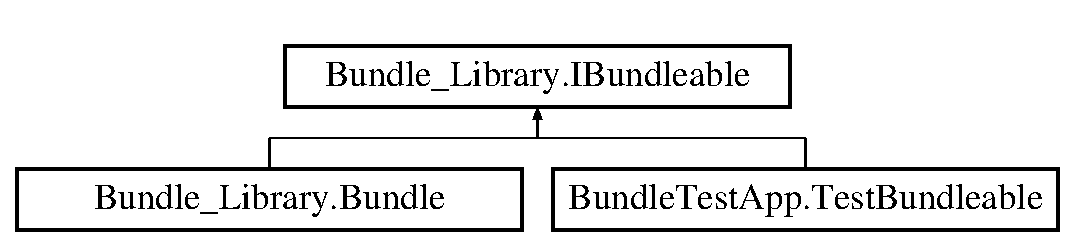
\includegraphics[height=2.000000cm]{interface_bundle___library_1_1_i_bundleable}
\end{center}
\end{figure}
\subsection*{Public Member Functions}
\begin{DoxyCompactItemize}
\item 
void {\bf pack\+Object} (string key, {\bf Bundle} B)
\begin{DoxyCompactList}\small\item\em Pack this object into a bundle \end{DoxyCompactList}\item 
{\bf I\+Bundleable} {\bf unpack\+Ooject} (string key, {\bf Bundle} B)
\begin{DoxyCompactList}\small\item\em Unpack this object from the bundle \end{DoxyCompactList}\end{DoxyCompactItemize}


\subsection{Detailed Description}
This interface allows objects to be packed in bundles. Any object you want to pack in a bundle must implement this interface 



\subsection{Member Function Documentation}
\index{Bundle\+\_\+\+Library\+::\+I\+Bundleable@{Bundle\+\_\+\+Library\+::\+I\+Bundleable}!pack\+Object@{pack\+Object}}
\index{pack\+Object@{pack\+Object}!Bundle\+\_\+\+Library\+::\+I\+Bundleable@{Bundle\+\_\+\+Library\+::\+I\+Bundleable}}
\subsubsection[{pack\+Object(string key, Bundle B)}]{\setlength{\rightskip}{0pt plus 5cm}void Bundle\+\_\+\+Library.\+I\+Bundleable.\+pack\+Object (
\begin{DoxyParamCaption}
\item[{string}]{key, }
\item[{{\bf Bundle}}]{B}
\end{DoxyParamCaption}
)}\label{interface_bundle___library_1_1_i_bundleable_a2257f911c2ef26f1d5586923bb2e036b}


Pack this object into a bundle 


\begin{DoxyParams}{Parameters}
{\em key} & the key that it will be stored with in the bundle\\
\hline
{\em B} & The bundle to pack it in\\
\hline
\end{DoxyParams}


Implemented in {\bf Bundle\+\_\+\+Library.\+Bundle} \doxyref{}{p.}{class_bundle___library_1_1_bundle_ad457ae404e0f33653d90ea5ed78287b4}.

\index{Bundle\+\_\+\+Library\+::\+I\+Bundleable@{Bundle\+\_\+\+Library\+::\+I\+Bundleable}!unpack\+Ooject@{unpack\+Ooject}}
\index{unpack\+Ooject@{unpack\+Ooject}!Bundle\+\_\+\+Library\+::\+I\+Bundleable@{Bundle\+\_\+\+Library\+::\+I\+Bundleable}}
\subsubsection[{unpack\+Ooject(string key, Bundle B)}]{\setlength{\rightskip}{0pt plus 5cm}{\bf I\+Bundleable} Bundle\+\_\+\+Library.\+I\+Bundleable.\+unpack\+Ooject (
\begin{DoxyParamCaption}
\item[{string}]{key, }
\item[{{\bf Bundle}}]{B}
\end{DoxyParamCaption}
)}\label{interface_bundle___library_1_1_i_bundleable_a9f33a8ca265623aa71e7a58fc9f398bd}


Unpack this object from the bundle 


\begin{DoxyParams}{Parameters}
{\em key} & the key that it was stored with in the bundle\\
\hline
{\em B} & The bundle that it is packed in\\
\hline
\end{DoxyParams}
\begin{DoxyReturn}{Returns}
the unpacked object from the bundle
\end{DoxyReturn}


Implemented in {\bf Bundle\+\_\+\+Library.\+Bundle} \doxyref{}{p.}{class_bundle___library_1_1_bundle_a7be22fd964ada1161611d764ded7381d}.



The documentation for this interface was generated from the following file\+:\begin{DoxyCompactItemize}
\item 
Bundle/I\+Bundleable.\+cs\end{DoxyCompactItemize}

\section{Bundle\+\_\+\+Library.\+Invalid\+Bundle\+Exception Class Reference}
\label{class_bundle___library_1_1_invalid_bundle_exception}\index{Bundle\+\_\+\+Library.\+Invalid\+Bundle\+Exception@{Bundle\+\_\+\+Library.\+Invalid\+Bundle\+Exception}}


This class represents an exception which is thrown when an invalid bundle has been used for a pack unpack operation  


Inheritance diagram for Bundle\+\_\+\+Library.\+Invalid\+Bundle\+Exception\+:\begin{figure}[H]
\begin{center}
\leavevmode
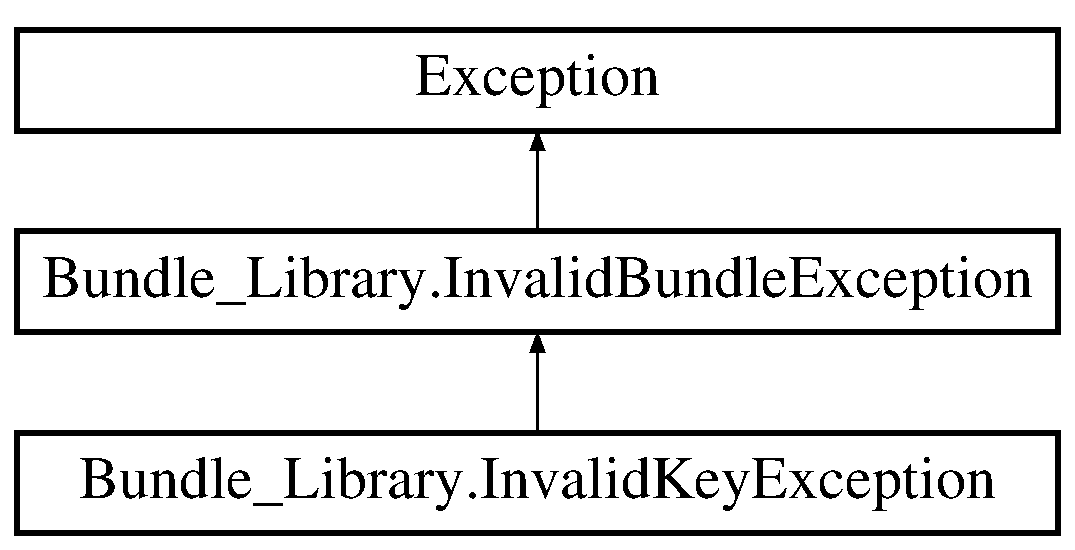
\includegraphics[height=3.000000cm]{class_bundle___library_1_1_invalid_bundle_exception}
\end{center}
\end{figure}
\subsection*{Public Member Functions}
\begin{DoxyCompactItemize}
\item 
{\bf Invalid\+Bundle\+Exception} ()
\begin{DoxyCompactList}\small\item\em Standard Constructor \end{DoxyCompactList}\item 
{\bf Invalid\+Bundle\+Exception} (string {\bf Message})
\begin{DoxyCompactList}\small\item\em Contructor which takes a message \end{DoxyCompactList}\end{DoxyCompactItemize}
\subsection*{Properties}
\begin{DoxyCompactItemize}
\item 
override string {\bf Message}\hspace{0.3cm}{\ttfamily  [get]}
\begin{DoxyCompactList}\small\item\em The default message displayed when the exception is thrown. This message is displayed if no message was passed in the constructor \end{DoxyCompactList}\end{DoxyCompactItemize}


\subsection{Detailed Description}
This class represents an exception which is thrown when an invalid bundle has been used for a pack unpack operation 



\subsection{Constructor \& Destructor Documentation}
\index{Bundle\+\_\+\+Library\+::\+Invalid\+Bundle\+Exception@{Bundle\+\_\+\+Library\+::\+Invalid\+Bundle\+Exception}!Invalid\+Bundle\+Exception@{Invalid\+Bundle\+Exception}}
\index{Invalid\+Bundle\+Exception@{Invalid\+Bundle\+Exception}!Bundle\+\_\+\+Library\+::\+Invalid\+Bundle\+Exception@{Bundle\+\_\+\+Library\+::\+Invalid\+Bundle\+Exception}}
\subsubsection[{Invalid\+Bundle\+Exception()}]{\setlength{\rightskip}{0pt plus 5cm}Bundle\+\_\+\+Library.\+Invalid\+Bundle\+Exception.\+Invalid\+Bundle\+Exception (
\begin{DoxyParamCaption}
{}
\end{DoxyParamCaption}
)}\label{class_bundle___library_1_1_invalid_bundle_exception_abf1e02c5e74b9350fcdb20ab8516cf00}


Standard Constructor 

\index{Bundle\+\_\+\+Library\+::\+Invalid\+Bundle\+Exception@{Bundle\+\_\+\+Library\+::\+Invalid\+Bundle\+Exception}!Invalid\+Bundle\+Exception@{Invalid\+Bundle\+Exception}}
\index{Invalid\+Bundle\+Exception@{Invalid\+Bundle\+Exception}!Bundle\+\_\+\+Library\+::\+Invalid\+Bundle\+Exception@{Bundle\+\_\+\+Library\+::\+Invalid\+Bundle\+Exception}}
\subsubsection[{Invalid\+Bundle\+Exception(string Message)}]{\setlength{\rightskip}{0pt plus 5cm}Bundle\+\_\+\+Library.\+Invalid\+Bundle\+Exception.\+Invalid\+Bundle\+Exception (
\begin{DoxyParamCaption}
\item[{string}]{Message}
\end{DoxyParamCaption}
)}\label{class_bundle___library_1_1_invalid_bundle_exception_adfa9d29595686208feee1defef15b9e0}


Contructor which takes a message 


\begin{DoxyParams}{Parameters}
{\em Message} & The message to display when the exception is thrown\\
\hline
\end{DoxyParams}


\subsection{Property Documentation}
\index{Bundle\+\_\+\+Library\+::\+Invalid\+Bundle\+Exception@{Bundle\+\_\+\+Library\+::\+Invalid\+Bundle\+Exception}!Message@{Message}}
\index{Message@{Message}!Bundle\+\_\+\+Library\+::\+Invalid\+Bundle\+Exception@{Bundle\+\_\+\+Library\+::\+Invalid\+Bundle\+Exception}}
\subsubsection[{Message}]{\setlength{\rightskip}{0pt plus 5cm}override string Bundle\+\_\+\+Library.\+Invalid\+Bundle\+Exception.\+Message\hspace{0.3cm}{\ttfamily [get]}}\label{class_bundle___library_1_1_invalid_bundle_exception_ad8726c1e618cb38e63240def5a57733e}


The default message displayed when the exception is thrown. This message is displayed if no message was passed in the constructor 



The documentation for this class was generated from the following file\+:\begin{DoxyCompactItemize}
\item 
Invalid\+Bundle\+Exception.\+cs\end{DoxyCompactItemize}

\section{Bundle\+\_\+\+Library.\+Invalid\+Key\+Exception Class Reference}
\label{class_bundle___library_1_1_invalid_key_exception}\index{Bundle\+\_\+\+Library.\+Invalid\+Key\+Exception@{Bundle\+\_\+\+Library.\+Invalid\+Key\+Exception}}


This class represents an exception which is thrown when the key was not found within the bundle  


Inheritance diagram for Bundle\+\_\+\+Library.\+Invalid\+Key\+Exception\+:\begin{figure}[H]
\begin{center}
\leavevmode
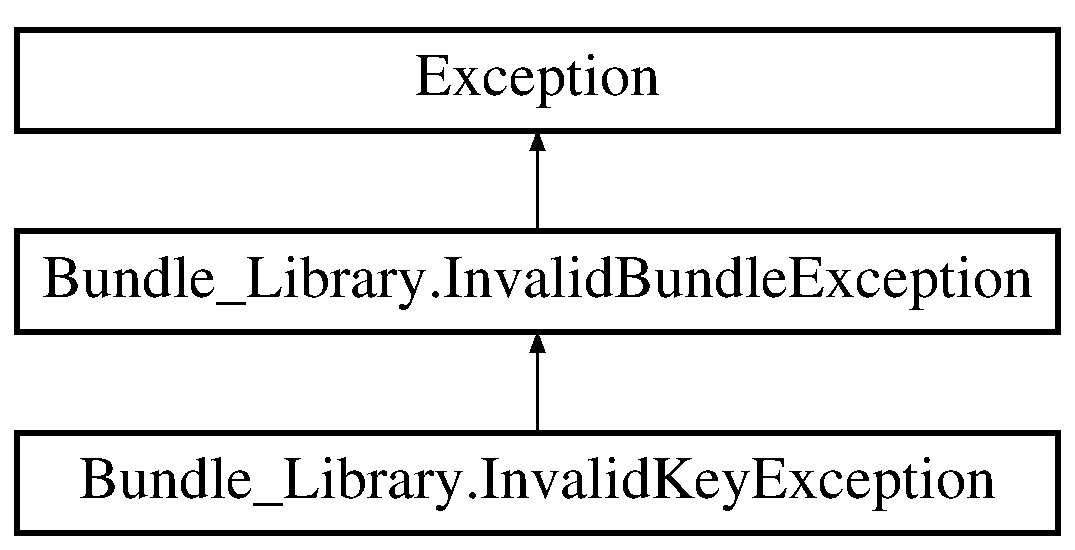
\includegraphics[height=3.000000cm]{class_bundle___library_1_1_invalid_key_exception}
\end{center}
\end{figure}
\subsection*{Public Member Functions}
\begin{DoxyCompactItemize}
\item 
{\bf Invalid\+Key\+Exception} ()
\begin{DoxyCompactList}\small\item\em Standard Constructor \end{DoxyCompactList}\item 
{\bf Invalid\+Key\+Exception} (string key)
\begin{DoxyCompactList}\small\item\em Contructor which takes a message \end{DoxyCompactList}\end{DoxyCompactItemize}
\subsection*{Properties}
\begin{DoxyCompactItemize}
\item 
string {\bfseries Key}\hspace{0.3cm}{\ttfamily  [get, set]}\label{class_bundle___library_1_1_invalid_key_exception_a78e11bc81fb6eb9a1a897256f806a357}

\item 
override string {\bf Message}\hspace{0.3cm}{\ttfamily  [get]}
\begin{DoxyCompactList}\small\item\em The default message displayed when the exception is thrown. This message is displayed if no message was passed in the constructor \end{DoxyCompactList}\end{DoxyCompactItemize}


\subsection{Detailed Description}
This class represents an exception which is thrown when the key was not found within the bundle 



\subsection{Constructor \& Destructor Documentation}
\index{Bundle\+\_\+\+Library\+::\+Invalid\+Key\+Exception@{Bundle\+\_\+\+Library\+::\+Invalid\+Key\+Exception}!Invalid\+Key\+Exception@{Invalid\+Key\+Exception}}
\index{Invalid\+Key\+Exception@{Invalid\+Key\+Exception}!Bundle\+\_\+\+Library\+::\+Invalid\+Key\+Exception@{Bundle\+\_\+\+Library\+::\+Invalid\+Key\+Exception}}
\subsubsection[{Invalid\+Key\+Exception()}]{\setlength{\rightskip}{0pt plus 5cm}Bundle\+\_\+\+Library.\+Invalid\+Key\+Exception.\+Invalid\+Key\+Exception (
\begin{DoxyParamCaption}
{}
\end{DoxyParamCaption}
)}\label{class_bundle___library_1_1_invalid_key_exception_a012627a068df2db2ae0f3d1284f9360d}


Standard Constructor 

\index{Bundle\+\_\+\+Library\+::\+Invalid\+Key\+Exception@{Bundle\+\_\+\+Library\+::\+Invalid\+Key\+Exception}!Invalid\+Key\+Exception@{Invalid\+Key\+Exception}}
\index{Invalid\+Key\+Exception@{Invalid\+Key\+Exception}!Bundle\+\_\+\+Library\+::\+Invalid\+Key\+Exception@{Bundle\+\_\+\+Library\+::\+Invalid\+Key\+Exception}}
\subsubsection[{Invalid\+Key\+Exception(string key)}]{\setlength{\rightskip}{0pt plus 5cm}Bundle\+\_\+\+Library.\+Invalid\+Key\+Exception.\+Invalid\+Key\+Exception (
\begin{DoxyParamCaption}
\item[{string}]{key}
\end{DoxyParamCaption}
)}\label{class_bundle___library_1_1_invalid_key_exception_af4f466d0dbea54778736377f282757fc}


Contructor which takes a message 


\begin{DoxyParams}{Parameters}
{\em Message} & The message to display when the exception is thrown\\
\hline
\end{DoxyParams}


\subsection{Property Documentation}
\index{Bundle\+\_\+\+Library\+::\+Invalid\+Key\+Exception@{Bundle\+\_\+\+Library\+::\+Invalid\+Key\+Exception}!Message@{Message}}
\index{Message@{Message}!Bundle\+\_\+\+Library\+::\+Invalid\+Key\+Exception@{Bundle\+\_\+\+Library\+::\+Invalid\+Key\+Exception}}
\subsubsection[{Message}]{\setlength{\rightskip}{0pt plus 5cm}override string Bundle\+\_\+\+Library.\+Invalid\+Key\+Exception.\+Message\hspace{0.3cm}{\ttfamily [get]}}\label{class_bundle___library_1_1_invalid_key_exception_a909f1ead8e9f50400f74338e7d27c0fa}


The default message displayed when the exception is thrown. This message is displayed if no message was passed in the constructor 



The documentation for this class was generated from the following file\+:\begin{DoxyCompactItemize}
\item 
Invalid\+Key\+Exception.\+cs\end{DoxyCompactItemize}

\section{Bundle\+Test\+App.\+Main\+Page Class Reference}
\label{class_bundle_test_app_1_1_main_page}\index{Bundle\+Test\+App.\+Main\+Page@{Bundle\+Test\+App.\+Main\+Page}}


An empty page that can be used on its own or navigated to within a Frame.  


Inheritance diagram for Bundle\+Test\+App.\+Main\+Page\+:\begin{figure}[H]
\begin{center}
\leavevmode
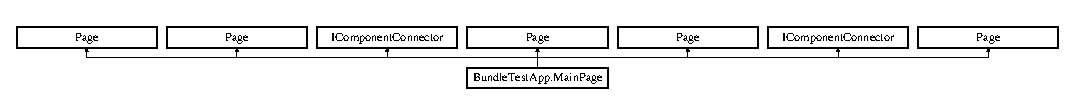
\includegraphics[height=0.963855cm]{class_bundle_test_app_1_1_main_page}
\end{center}
\end{figure}
\subsection*{Public Member Functions}
\begin{DoxyCompactItemize}
\item 
void {\bfseries Connect} (int connection\+Id, object target)\label{class_bundle_test_app_1_1_main_page_a1b2894ce672e07a268d1a08b1ccad0ee}

\item 
void {\bfseries Initialize\+Component} ()\label{class_bundle_test_app_1_1_main_page_ae952fc1d1b7431744de6901a59ebdd5f}

\item 
void {\bfseries Connect} (int connection\+Id, object target)\label{class_bundle_test_app_1_1_main_page_a1b2894ce672e07a268d1a08b1ccad0ee}

\item 
void {\bfseries Initialize\+Component} ()\label{class_bundle_test_app_1_1_main_page_ae952fc1d1b7431744de6901a59ebdd5f}

\end{DoxyCompactItemize}
\subsection*{Protected Member Functions}
\begin{DoxyCompactItemize}
\item 
override void {\bf On\+Navigated\+To} (Navigation\+Event\+Args e)
\begin{DoxyCompactList}\small\item\em Invoked when this page is about to be displayed in a Frame. \end{DoxyCompactList}\end{DoxyCompactItemize}


\subsection{Detailed Description}
An empty page that can be used on its own or navigated to within a Frame. 



\subsection{Member Function Documentation}
\index{Bundle\+Test\+App\+::\+Main\+Page@{Bundle\+Test\+App\+::\+Main\+Page}!On\+Navigated\+To@{On\+Navigated\+To}}
\index{On\+Navigated\+To@{On\+Navigated\+To}!Bundle\+Test\+App\+::\+Main\+Page@{Bundle\+Test\+App\+::\+Main\+Page}}
\subsubsection[{On\+Navigated\+To(\+Navigation\+Event\+Args e)}]{\setlength{\rightskip}{0pt plus 5cm}override void Bundle\+Test\+App.\+Main\+Page.\+On\+Navigated\+To (
\begin{DoxyParamCaption}
\item[{Navigation\+Event\+Args}]{e}
\end{DoxyParamCaption}
)\hspace{0.3cm}{\ttfamily [protected]}}\label{class_bundle_test_app_1_1_main_page_a07b7fa2266245c00e301a2c32a4ceb92}


Invoked when this page is about to be displayed in a Frame. 


\begin{DoxyParams}{Parameters}
{\em e} & Event data that describes how this page was reached. This parameter is typically used to configure the page.\\
\hline
\end{DoxyParams}


The documentation for this class was generated from the following files\+:\begin{DoxyCompactItemize}
\item 
D\+:/\+Git\+Hub/\+Windows-\/\+Phone-\/\+Bundle/\+Bundle\+Test\+App/Main\+Page.\+xaml.\+cs\item 
D\+:/\+Git\+Hub/\+Windows-\/\+Phone-\/\+Bundle/\+Bundle\+Test\+App/obj/\+Debug/Main\+Page.\+g.\+i.\+cs\item 
D\+:/\+Git\+Hub/\+Windows-\/\+Phone-\/\+Bundle/\+Bundle\+Test\+App/obj/\+Debug/Main\+Page.\+g.\+cs\end{DoxyCompactItemize}

\section{Bundle\+\_\+\+Library.\+Test\+Bundleable Class Reference}
\label{class_bundle___library_1_1_test_bundleable}\index{Bundle\+\_\+\+Library.\+Test\+Bundleable@{Bundle\+\_\+\+Library.\+Test\+Bundleable}}


This class represents a simple object that can be packed and unpacked from a bundle.  


Inheritance diagram for Bundle\+\_\+\+Library.\+Test\+Bundleable\+:\begin{figure}[H]
\begin{center}
\leavevmode
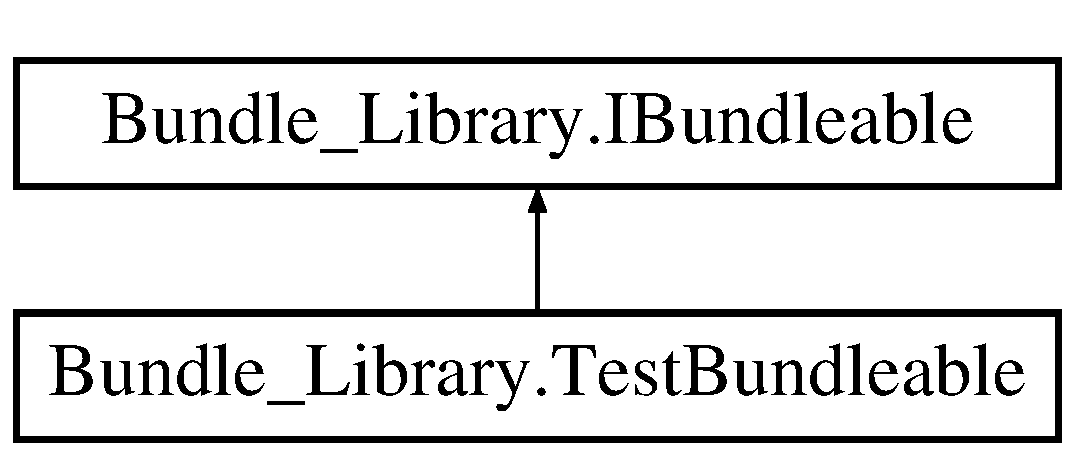
\includegraphics[height=2.000000cm]{class_bundle___library_1_1_test_bundleable}
\end{center}
\end{figure}
\subsection*{Public Member Functions}
\begin{DoxyCompactItemize}
\item 
{\bf Test\+Bundleable} ()
\begin{DoxyCompactList}\small\item\em Contructor for this object \end{DoxyCompactList}\end{DoxyCompactItemize}
\subsection*{Properties}
\begin{DoxyCompactItemize}
\item 
string {\bfseries Test\+String}\hspace{0.3cm}{\ttfamily  [get, set]}\label{class_bundle___library_1_1_test_bundleable_a70e5ac66f3a95dc108ab1cf510bbc5ae}

\item 
int {\bfseries Test\+Int}\hspace{0.3cm}{\ttfamily  [get, set]}\label{class_bundle___library_1_1_test_bundleable_ac9c62b50e4b1d8358addb26d3a007b0c}

\end{DoxyCompactItemize}


\subsection{Detailed Description}
This class represents a simple object that can be packed and unpacked from a bundle. 



\subsection{Constructor \& Destructor Documentation}
\index{Bundle\+\_\+\+Library\+::\+Test\+Bundleable@{Bundle\+\_\+\+Library\+::\+Test\+Bundleable}!Test\+Bundleable@{Test\+Bundleable}}
\index{Test\+Bundleable@{Test\+Bundleable}!Bundle\+\_\+\+Library\+::\+Test\+Bundleable@{Bundle\+\_\+\+Library\+::\+Test\+Bundleable}}
\subsubsection[{Test\+Bundleable()}]{\setlength{\rightskip}{0pt plus 5cm}Bundle\+\_\+\+Library.\+Test\+Bundleable.\+Test\+Bundleable (
\begin{DoxyParamCaption}
{}
\end{DoxyParamCaption}
)}\label{class_bundle___library_1_1_test_bundleable_adb459e6fb5df725d58aad7ad9408d01b}


Contructor for this object 



The documentation for this class was generated from the following file\+:\begin{DoxyCompactItemize}
\item 
Bundle/Test\+Bundleable.\+cs\end{DoxyCompactItemize}

%--- End generated contents ---

% Index
\backmatter
\newpage
\phantomsection
\clearemptydoublepage
\addcontentsline{toc}{chapter}{Index}
\printindex

\end{document}
